%!TEX root = thesis.tex
\chapter{Interconnect}
\label{sec:interconnect}
ReconOS provides exceptional transparency regarding the implementation and
execution mode of a thread over the hardware/software boundary. However, the
delegate mechanism introduces an overhead for communication between threads
running in hardware. While for computational intensive tasks with low
communication demand the overhead is acceptable, for low-latency applications
with real-time aspects it breaks the overall performance significantly.
Especially for \acp{PAC}, utilizing the \ac{FPGA} for low-latency and
performance critical parts of the controller, a fast communication is crucial.

This section addresses the topic of communication overhead and investigates
ways to speedup the on-chip communication without loosing transparency or
burden the developer with additional tasks. Starting with a short evaluation
of the current system, different approaches compared to the literature are
discussed. The final architecture is then implemented and evaluated.

\section{Evaluation of the current System}
While the basic concepts of the delegate mechanism were already discussed in
the previous section, a detailed knowledge of its implementation and
performance limitations is required. Consider figure \ref{fig:delegate},
showing a detailed view of the delegate implementation, consisting out of
communication interfaces, interrupt lines and drivers.
\begin{figure}
	\centering
	%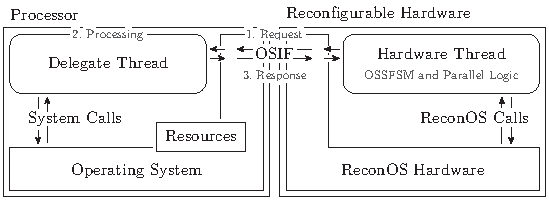
\includegraphics[width=6cm]{../figures/delegate}
	\caption{ReconOS delegate mechanism in detail}
	\label{fig:delegate}
\end{figure}
 The \ac{OSIF} connects the hardware slot with the delegate thread as a
bidirectional \ac{FIFO} interface and allows message based communication. The
\acp{FIFO} are implemented in the reconfigurable fabric and attached to the
\ac{AXI} bus via an interface bridge. It provides access from the \ac{CPU} by
a set of memory mapped register for each \ac{OSIF} and allows to read status
bits or data words. Since the delegate threads waiting for requests from the
hardware threads should not consume processing time on the processor, they are
blocked and waiting for an interrupt. Since a  normal process in Linux is not
allowed to register interrupt handlers, a driver handles all kernel specific
features and provides an interface to the user space.

To illustrate the procedure of delegating an \ac{OS} call, figure
\ref{fig:delegate} sketches an exemplary \lstinline{MBOX_GET}. At first, the
hardware thread issues the request by writing messages into the \ac{OSIF},
namely an internal encoding of the command followed by an identification of
the appropriate \ac{OS} resource and additional arguments. The interrupt
causes the delegate thread to wake up, read the messages from the \ac{OSIF}
and decode the commands. After executing the appropriate \ac{OS} call, the
delegate thread writes back an acknowledge into the \ac{OSIF} and, optionally,
the result of the system call. Following this process, the exchange of a
single message between two hardware threads via a mailbox includes two
interrupts implying context switches into the kernel space, the handling of
the mailbox by the kernel and the access of the \ac{OSIF}. All these
operations take, comparing to a directly in hardware implemented communication
mechanism, a significantly longer period and burden the processor with
additional tasks. Table \ref{tab:delegate_old} shows the turnaround times of
different \ac{OS} calls averaged over 1024 executions, for example, the time
needed to propagate a message via a mailbox or synchronize via a mutex.
\begin{table}[ht]
	\centering
	\renewcommand{\arraystretch}{1.2}
	\begin{tabular}{l r r r r}
		\hline
		Dir & sem & mutex & cond  & mbox\\
		\hline
		\hline
		H-H & 2019 & 2012 & 2080 & 2235\\
		H-S & 1937 & 1932 & 1997 & 2161\\
		S-H & 1638 & 1632 & 1702 & 1715\\
		S-S & 1523 & 1521 & 1610 & 1643\\
		\hline
	\end{tabular}
	\caption{Turnaround times of OSIF functions in clock cycles of 100MHz}
	\label{tab:delegate_old}
\end{table}
While these measurements were made under a low load and no other communication
present, a real world application would be much worse. \todo{make new
measurements under load}

\section{Architectural Considerations}
To speedup the communication, provide low-latency communication and reduce the
load of the main processor, a direct communication between hardware threads
becomes necessary. However, such a communication infrastructure should be
automatically handled by the ReconOS runtime and abstracted by the known
\ac{OS} interfaces, to provide an unchanged interface and do not lose any of
the exceptional transparency.

Besides ReconOS, there exist other operating systems leveraging the
multithreaded programming model and providing a transparent interface. The
most important and comparable framework is the hthreads project, focusing on
low-jitter hardware implementations of \ac{OS} functions \citep{AHK14}. It
provides similar functionality but follows a different approach as illustrated
by the block diagram in figure \ref{fig:hthreads}.
\begin{figure}
	\centering
	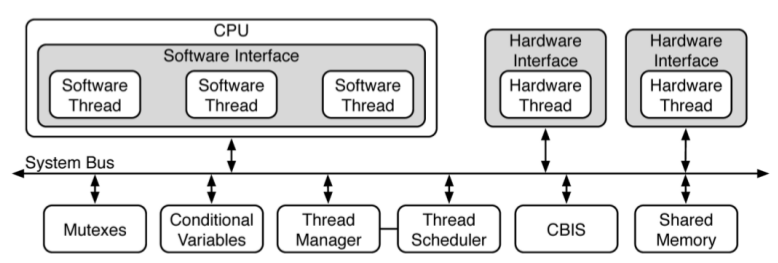
\includegraphics[width=6cm]{../figures/hthreads}
	\caption{Hthreads system block diagram \citep{ASA08}}
	\label{fig:hthreads}
\end{figure}
Instead of utilizing an existing \ac{OS} and its functions through a delegate
mechanism, it implements all resources together with scheduling and management
components in the reconfigurable fabric \citep{ASA08}. While this guarantees a
low-latency access to all components, the central system bus limits the
overall performance in high-load situation. Furthermore, the architecture
makes it unportable to standard \ac{OS} kernels or other platforms.

A direct inter-thread communication implemented in hardware seems to be
necessary, to provide a fast and low-latency communication. Adopting the idea
of implementing \ac{OS} functions on the \ac{FPGA} for the ReconOS framework
promises significant speedups for many applications and seems to be crucial to
utilize ReconOS in modern \ac{PAC} designs. However, the key benefits of
ReconOS must be maintained, for example the exceptional transparency regarding
implementation of threads, the portability and interoperability through
standard \ac{OS} kernels or the simple tool flow. For the developer, the
internal implementation of resources and the selection of appropriate
communication mechanisms should be completely hidden and handled
automatically.

\begin{itemize}
\item Motivation for interconnect (experiments, other projects, ...)
\item Always via software to slow
\item Consideration (resource limitations, ...)
\item Reconfigurable later on?
\end{itemize}
\begin{itemize}
\item Comparison of different approaches
\item HThreads, ...?
\end{itemize}
\section{Implementation}
\section{Evaluation}
\begin{itemize}
\item measure time differences for old/new
\item show speedup/speeddown
\end{itemize}